\documentclass[10pt, a4paper]{article}

%\usepackage[paper=a4paper, left=1.5cm, right=1.5cm, bottom=1.5cm, top=3.5cm]{geometry}
\usepackage[paper=a4paper]{geometry}
\usepackage[latin1]{inputenc}
\usepackage[T1]{fontenc}
\usepackage[spanish]{babel}
\usepackage{indentfirst}
\usepackage{fancyhdr}
\usepackage{latexsym}
\usepackage{lastpage}
\usepackage[colorlinks=true, linkcolor=blue]{hyperref}
\usepackage{calc}
\usepackage{paralist}
\usepackage{caratula}
%\usepackage[plain,noline,linesnumberedhidden, noend]{algorithm2e}
%\usepackage[plain,noline,linesnumbered, noend]{algorithm2e}
\usepackage[plain,noline,noend]{algorithm2e}
\usepackage{graphicx}
\usepackage{caption}
\usepackage{subcaption}
\usepackage{amsmath}
\usepackage{float}

\newcommand{\f}[1]{\text{#1}}
\newcommand{\call}[1] {\textsc{#1}}
\newcommand{\tab}[1]{\Indp \Indp #1 \Indm  \Indm}
\newcommand{\tabSpace}[1]{\Indp \Indp \; #1 \Indm \Indm \;}
\newcommand{\si}[2]{ {\bf si} (#1)\; \tab {#2} }
\newcommand{\sino}[1]{ {\bf sino}\; \tab {#1} }
\newcommand{\sinosi}[2]{ {\bf sino, si #1}\; \tab {#2} }
\newcommand{\mientras}[2] {  {\bf mientras} (#1) \; \tabSpace  {#2} }
\newcommand{\funcion}[3] { 	\KwSty{\call{#1}(#2)}\; \tabSpace  {#3} \KwSty{\call{Fin Funcion}} \newline }
\newcommand{\funcionConResultado}[4] {      \KwSty{\call{#1}(#2) $\rightarrow$ #3}\; \tabSpace  {#4} \KwSty{\call{Fin Funcion}} \newline }
\newcommand{\porcada}[3] { {\bf por cada } #1 {\bf en} #2 \; \tabSpace {#3} }
\newcommand{\para}[4] { {\bf para } #1 {\bf desde} #2 {\bf hasta} #3\; \{ \; \tab{#4}\}\; }
\newcommand{\paracada}[3] { {\bf para cada } #1 {\bf $\in$} #2 \; \tabSpace {#3} }
\newcommand{\devolver}[1] { {\bf devolver} #1\;}



\sloppy


\hypersetup{%
 % Para que el PDF se abra a pagina completa.
 pdfstartview= {FitH \hypercalcbp{\paperheight-\topmargin-1in-\headheight}},
 pdfauthor={C\'atedra de Algoritmos y Estructuras de Datos III - DC - UBA},
 pdfkeywords={Trabajo Pr\'actico 3},
 pdfsubject={}
}

\parskip=5pt % 10pt es el tama\~no de fuente

% Pongo en 0 la distancia extra entre itemes.
\let\olditemize\itemize
\def\itemize{\olditemize\itemsep=0pt}

% Acomodo fancyhdr.
\pagestyle{fancy}
\thispagestyle{fancy}
\addtolength{\headheight}{1pt}
\lhead{Base de Datos}
\rhead{TP1}
\cfoot{\thepage /\pageref{LastPage}}
\renewcommand{\footrulewidth}{0.4pt}

\author{Base de Datos, DC, UBA.}
\date{}
\title{}

\begin{document}

%Pagina de titulo e indice
\thispagestyle{empty}
\materia{Base de datos}
\submateria{TP1}
\titulo{}
\grupo{NN\_3}
\integrante{Sergio Gonz\'alez}{723/10}{sergiogonza90@gmail.com}
\integrante{Gino Scarpino}{392/08}{gino.scarpino@gmail.com}
\maketitle

\tableofcontents

\SetAlgoSkip{bigskip}
\NoCaptionOfAlgo
\DontPrintSemicolon
\SetAlFnt{\ttfamily}

\newpage

\section{Introduccion}

	La intenci\'on de este trabajo pr\'actico es implementar una soluci\'on a un problema de modelado, utilizando los conceptos aprendidos durante esta etapa de la materia. \\
En esta ocasi\'on el problema a modelar es el funcionamiento de las c�maras legislativas, si bien no es un funcionamiento exacto como el de la Rep\'ublica Argentina, el enunciado consiste en una aproximaci\'on. \\
Dado que el enunciado mismo presentaba algunas ambig�edades o bien otorgaba libertades a la hora de modelar, las condiciones asumidas se explicar\'an en una secci\'on posterior, cabe resaltar que todo fue consultado con los docentes de la c\'atedra. \\


 
\section{Modelo entidad Relaci\'on}

Para hacer el modelo utilizamos la notacion vista en la catedra, excepto por las carnalidades donde se representan de manera distinta, as\'i por ejemplo una relaci\'on M:N sera algo de la forma:

\begin{figure}[ht]
  \begin{center}
    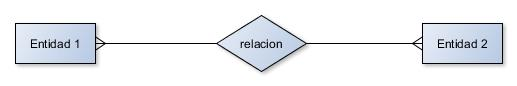
\includegraphics[scale=.75]{./imagenes/ejrelacion.jpg}
    \caption{relacion M:N} 
    \label{fig:graficomn}
  \end{center}
\end{figure}

Una relacion N:1 sera algo de la forma:

\begin{figure}[ht]
  \begin{center}
    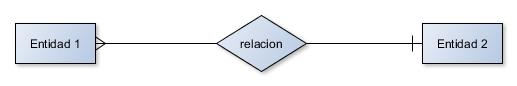
\includegraphics[scale=.75]{./imagenes/ejrelacion2.jpg}
    \caption{relacion N:1} 
    \label{fig:grafico}
  \end{center}
\end{figure}

\section{Diagrama Entidad Relaci\'on (DER)}

	\subsection{Breve descripcion de las entidades}
	%%%%% ESTE PUNTO FUE UNA DE LAS CORRECCIONES, AGREGAR UNA DESCRIPCION DE CADA ENTIDADE NO TRIVIAL. %%%%%%

		bla bla

	\newpage
	\subsection{DER}

		Separamos el gráfico en dos fragmentos de manera de hacerlo más legible, ambas partes pueden leerse de manera independiente y están centradas en la entidad Legislador.
			
		\begin{figure}[ht]
		  %\begin{center}
		    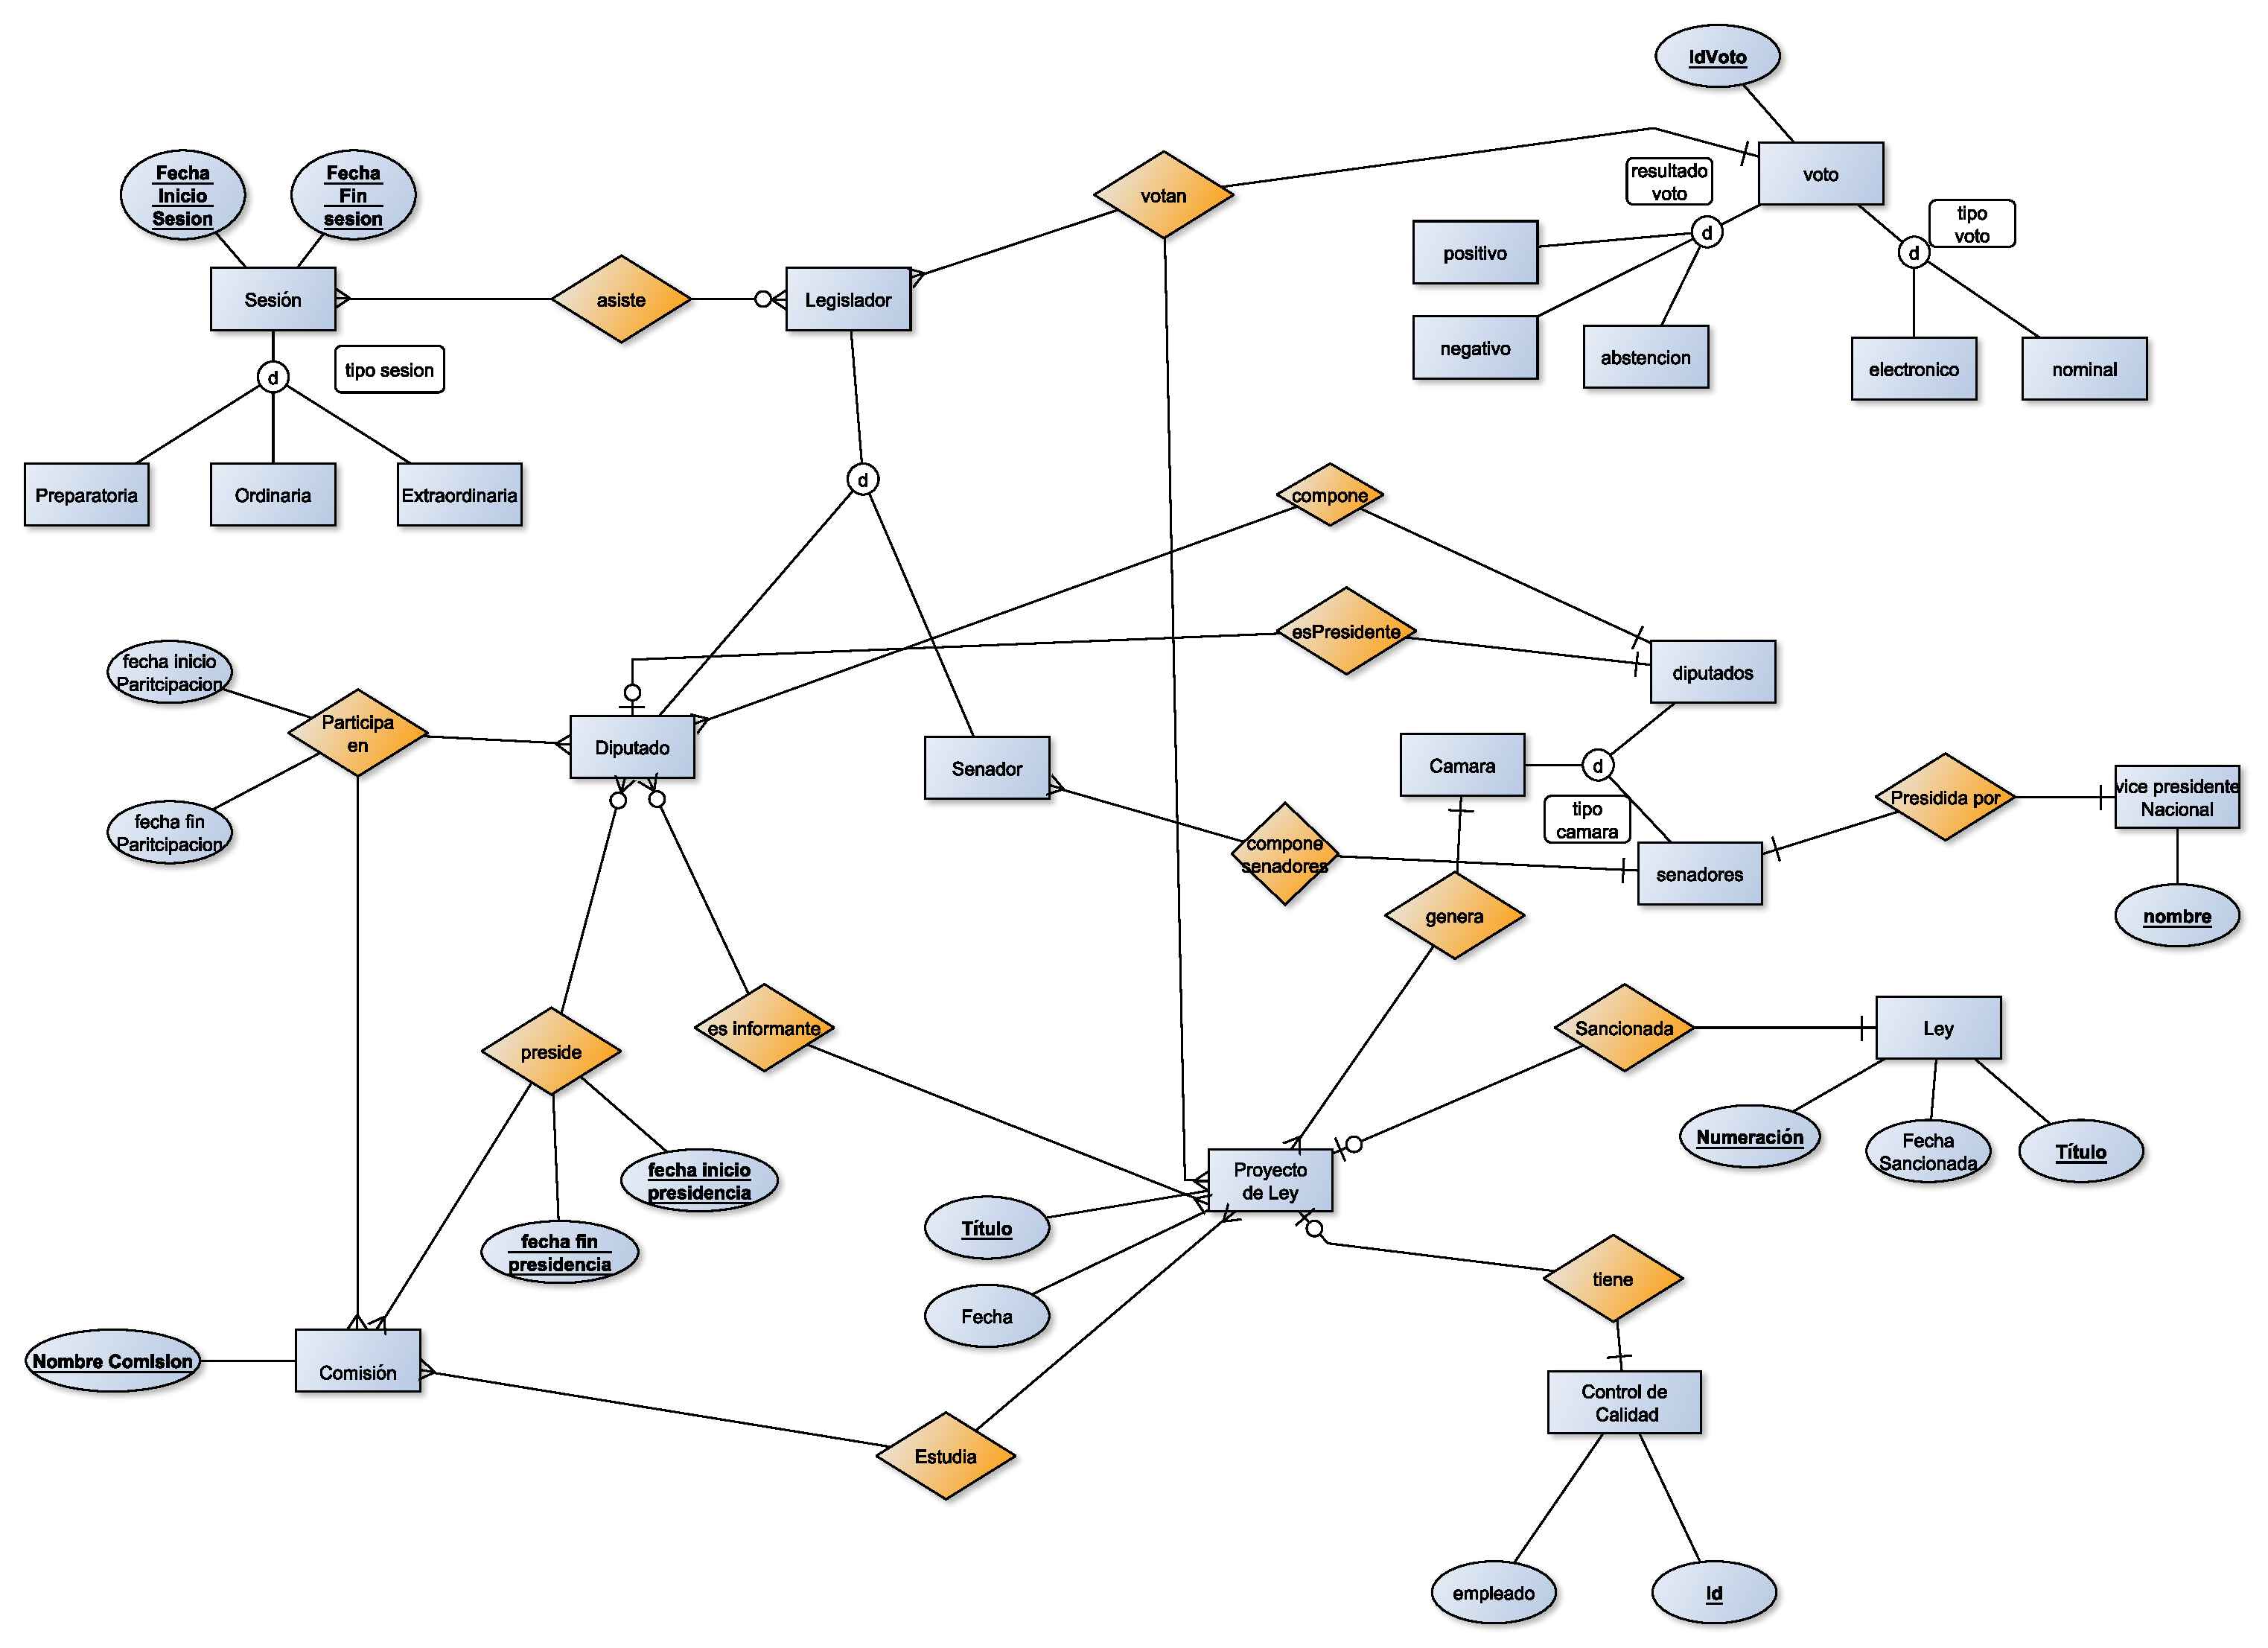
\includegraphics[scale=.30]{./imagenes/DERParteDeAbajo.pdf}
		    \caption{fragmento der} 
		    \label{fig:derparte1}
		  %\end{center}
		\end{figure}
				
		\begin{figure}[ht]
		  %\begin{center}
		    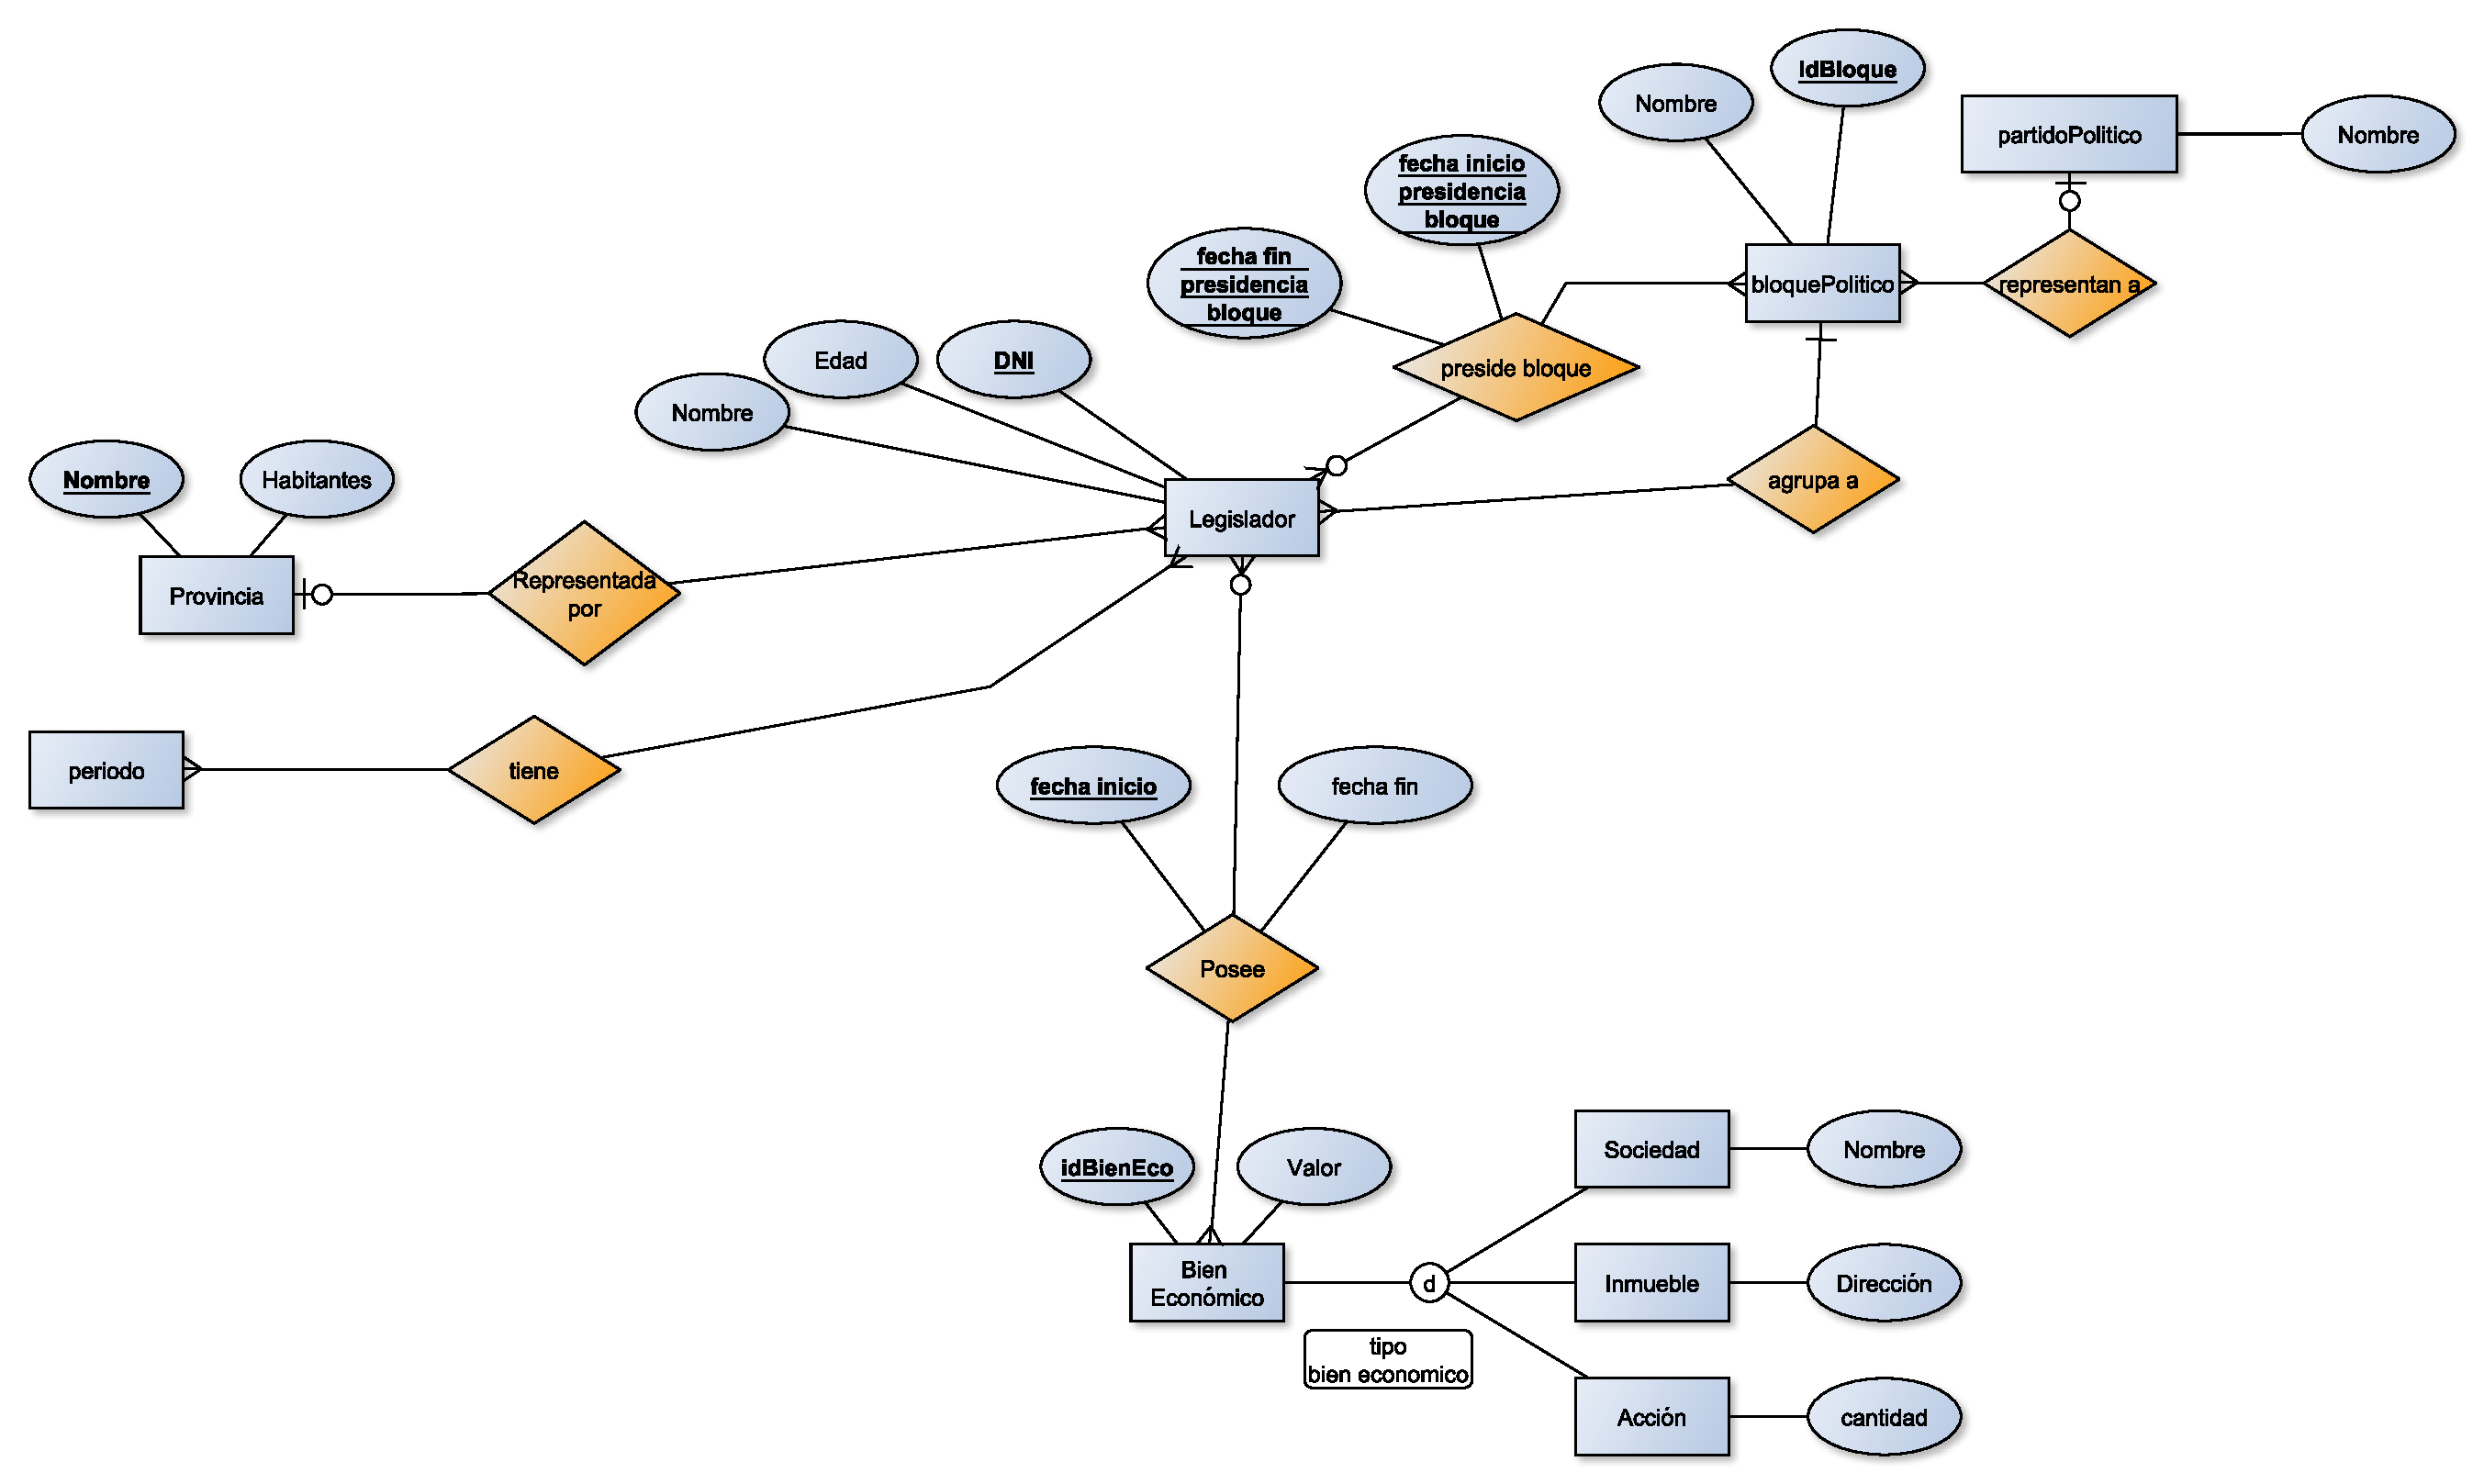
\includegraphics[scale=.30]{./imagenes/DERParteDeArriba.pdf}
		    \caption{fragmento der segunda parte} 
		    \label{fig:derparte2}
		  %\end{center}
		\end{figure}

	\newpage
	\subsection{Restricciones}
	
		\begin{itemize}
	\item El atributo edad de cada legislador que sea diputado es de por lo menos 25.
	\item El atributo edad  de cada legislador en la c\'amara de senadores es de al menos 30.
	\item En la c\'amara de senadores no puede haber ni mas ni menos de 3 representantes por provincia.
	\item La fecha de inicio de cargo de ser menor a la fecha de fin de cargo.
	\item No puede haber un legislador que sea legislador y diputado en periodos de
	 inicio de periodo y fin periodo solapados.
	
	\item En todas las relaciones que tengan fechas como atributos las fechas de inicio
	 deben ser anteriores a las de fin.
	
	\item La cantidad de comisiones que la c\'amara de diputados es de 45.
	
	\item La fecha de una inicio y fin de una sesi\'on puede estar entre el 1 de marzo al 30 de noviembre de un mismo a\~no.
	
	\item La suma de los votos totales de un proyecto de ley aprobado es igual a la suma de todos los legisladores que son diputados y todos los legisladores que son senadores, que estuvieron presentes en las sesiones.
	
	\item Todos los legisladores que componen la c\'amara de diputados, son diputados y todos los que componen la c\'amara de senadores son senadores.
	
	\item La cantidad de senadores en la c\'amara de senadores es de 3\* cantidad de provincias.
	
	\item La cantidad de legisladores que asiste a cada sesi\'on es menor o igual a la cantidad de legisladores que componen la c\'amara de diputados o la cantidad de legisladores que componen la c\'amara senadores.
	
	\item Si un legislador ``l'' tiene mas de 15 ausencias hasta determinada fecha, entonces no puede haber una tupla de la forma (l,s) en la relaci\'on asiste donde ``s'' es una sesi\'on, con fecha dentro del periodo de actividad del legislador.
	
	\item Los atributos fecha de inicio y fecha fin de participaci\'on en comisiones, presidencia de bloques o bien presidencia de comisiones deben estar incluidas en el periodo de de inicio y fin que tiene como legislador.
	
	\item Si un diputado d, preside una comisi\'on c, en una fecha de inicio i, y fin d. Entonces no existen dos tuplas t1 y t2 en la relaci\'on preside de la forma(d,c) con fechas de inicio y fin solapadas. Es decir un diputado solo puede presidir una comisi\'on a la vez.


\end{itemize}	

\end{document}